En este capítulo se presenta una descripción detallada del conjunto de datos BugHunter, incluyendo su origen, estructura, y una descripción exhaustiva de sus características (métricas de código) y tamaño. Se detallan las herramientas y técnicas empleadas, así como las distintas etapas del proceso de selección de características. Finalmente, se describe el procedimiento adoptado para llevar a cabo los experimentos, incluyendo los pasos seguidos para entrenar y validar los modelos.

\section{BUGHUNTER}


Utilizamos el Conjunto de datos BugHunter: un tipo novedoso de conjunto de datos de errores construido automáticamente y disponible gratuitamente que contiene elementos de código (archivos, clases, métodos) con un amplio conjunto de métricas de código e información de errores \cite{ferenc_automatically_2020}.

Otros conjuntos de datos de errores disponibles siguen el enfoque tradicional (PROMISE \cite{sayyad_shirabad_promise_2005}, Eclipse, entre otros) de recopilar las características de todos los elementos del código fuente (con errores y sin errores) en solo una o más versiones de lanzamiento preseleccionadas del código. El enfoque seleccionado, por otro lado, captura el error y los estados fijos de los mismos elementos del código fuente desde el marco de tiempo más estrecho que podemos identificar para detectar la presencia de un error, independientemente de las versiones de lanzamiento.

El conjunto de datos contiene información útil de caracterización de elementos de código defectuoso, se utilizan varios proyectos almacenados en GitHub que son mantenidos regularmente. Se utiliza la API de GitHub que hace posible implementar una herramienta de recuperación automática de datos. Se seleccionan 15 proyectos Java como sistemas temáticos, que difieren en muchos aspectos entre sí (tamaño, dominio, número de errores informados) para cubrir un conjunto amplio y general de sistemas \cite{ferenc_automatically_2020}. 

El conjunto de datos se basa en un nuevo enfoque que recopila información del instante antes y después de la corrección de los elementos del código fuente (y sus características) que se vieron afectados por errores y no considera aquellos elementos del código que no fueron afectados por errores. Este tipo de conjunto de datos ayuda a capturar los cambios en las métricas de los productos de software cuando se corrige un error. Por lo tanto, se puede aprender de las diferencias en las métricas del código fuente entre elementos de código defectuosos y no defectuosos.

En la tabla \ref{table:datasetmeta}, resumimos los metadatos principales del conjunto de datos. La cantidad de métricas existentes en cada categoría y la cantidad de registros existentes en cada uno de los niveles de granularidad.

\begin{table}[H]
\captionsetup{labelsep=period, labelfont=bf}
\caption{Metadatos del conjunto de datos}
\centering
\begin{tabular}{lc}
\toprule
\textbf{Granularity}        & file, class, method                                                                                                                \\\midrule
\textbf{Number of projects} & 15                                                                                                                                 \\ 
\hline
\textbf{Number of metrics}  & \begin{tabular}[c]{@{}c@{}}static source code metrics (66),\\ code duplication metrics (8),\\ code smell metrics (35)\end{tabular} \\
\hline
\textbf{Number of entries}  & \begin{tabular}[c]{@{}c@{}}file: 70,088\\ class: 84,562\\ method: 159,078


\end{tabular}  
\\\bottomrule
\end{tabular}

\label{table:datasetmeta}
\end{table} 

 Realizamos una descripción de los datos en \ref{description-table} mostrando cantidad, media, desviación estándar, mínimo, máximo y cantidad de elementos. Al analizar la tabla descriptiva de los datos podemos concluir:
 {
\fontsize{14pt}{14pt}\selectfont
\begin{itemize}
\item No existen datos nulos dado que el contados de todos es igual al total de registros.
\item Gran variedad en los rangos de los datos.
\item Una gran cantidad de características que tienen moda y mediana iguales y con valor 0, pudiendo implicar poca variación en sus datos.
\end{itemize}
}

El conjunto de datos BugHunter cuenta con varias métricas de código extraídas con la herramienta OpenStaticAnalyzer \cite{openstaticanalyzergithubio} utilizando el código etiquetado en el GitHub de 15 proyectos, escritos en Java. Especialmente los más grandes y que tengan una cantidad adecuada de problemas etiquetados como errores, porque son más adecuados para este tipo de análisis.

\begin{table}[H]
{
\captionsetup{labelsep=period, labelfont=bf}
\caption{ Description Table}
\fontsize{9pt}{6pt}\selectfont
\begin{tabular}{@{}lp{10mm}p{10mm}p{10mm}p{10mm}llllll@{}} 
\toprule
Medida& Media & Error   típico & Mediana & Moda & Desviación   estándar & Varianza   de la muestra & Mínimo & Máximo & Suma& Cuenta \\ 
\midrule
CC                                  & 0,12           & 0,00                    & 0,00             & 0,00          & 0,30                           & 0,09                              & 0,00            & 1,00            & 19334,08       & 159078,00       \\
CCL                                 & 0,66           & 0,03                    & 0,00             & 0,00          & 11,53                          & 133,02                            & 0,00            & 499,00          & 104713,00      & 159078,00       \\
CCO                                 & 4,01           & 0,71                    & 0,00             & 0,00          & 282,97                         & 80069,76                          & 0,00            & 75248,00        & 638669,00      & 159078,00       \\
CI                                  & 1,95           & 0,14                    & 0,00             & 0,00          & 56,22                          & 3160,84                           & 0,00            & 4671,00         & 310335,00      & 159078,00       \\
CLC                                 & 0,12           & 0,00                    & 0,00             & 0,00          & 0,30                           & 0,09                              & 0,00            & 1,00            & 19071,79       & 159078,00       \\
LDC                                 & 7,52           & 0,37                    & 0,00             & 0,00          & 146,09                         & 21343,22                          & 0,00            & 6691,00         & 1196598,00     & 159078,00       \\
LLDC                                & 6,72           & 0,33                    & 0,00             & 0,00          & 132,41                         & 17531,44                          & 0,00            & 5848,00         & 1068422,00     & 159078,00       \\
HCPL                                & 202,83         & 1,94                    & 106,09           & 13,61         & 771,92                         & 595862,35                         & 2,00            & 57839,10        & 32266128,82    & 159078,00       \\
HDIF                                & 26,30          & 0,96                    & 15,04            & 3,50          & 384,17                         & 147587,63                         & 1,00            & 56556,50        & 4183142,22     & 159078,00       \\
HEFF                                & 250671,02      & 65265,39                & 3554,80          & 49,13         & 26030828,33                    & 677604023793090,00                & 4,75            & 3944690000,00   & 39876245063,67 & 159078,00       \\
HNDB                                & 910,90         & 43,12                   & 232,92           & 13,41         & 17198,86                       & 295800753,28                      & 2,83            & 2496560,00      & 144904764,53   & 159078,00       \\
HPL                                 & 120,57         & 2,12                    & 48,00            & 12,00         & 844,70                         & 713519,30                         & 3,00            & 39378,00        & 19180331,00    & 159078,00       \\
HPV                                 & 39,73          & 0,19                    & 27,00            & 10,00         & 74,43                          & 5539,97                           & 3,00            & 4764,00         & 6319883,00     & 159078,00       \\
HTRP                                & 13926,17       & 3625,86                 & 197,49           & 2,73          & 1446157,65                     & 2091371943879,64                  & 0,26            & 219150000,00    & 2215347324,87  & 159078,00       \\
HVOL                                & 848,92         & 23,68                   & 230,00           & 19,65         & 9444,64                        & 89201173,08                       & 4,75            & 451128,00       & 135044408,26   & 159078,00       \\
MI                                  & 104,36         & 0,06                    & 106,10           & 132,83        & 23,81                          & 567,01                            & -579,07         & 162,66          & 16602174,03    & 159078,00       \\
MIMS                                & 61,05          & 0,03                    & 62,05            & 77,68         & 13,74                          & 188,78                            & 0,00            & 95,12           & 9712500,44     & 159078,00       \\
MISEI                               & 83,11          & 0,08                    & 84,46            & 116,03        & 33,76                          & 1139,90                           & -668,08         & 208,70          & 13221672,48    & 159078,00       \\
MISM                                & 48,73          & 0,05                    & 49,39            & 67,85         & 19,25                          & 370,44                            & 0,00            & 122,05          & 7751585,71     & 159078,00       \\
McCC                                & 3,54           & 0,03                    & 1,00             & 1,00          & 12,08                          & 146,02                            & 1,00            & 2387,00         & 562498,00      & 159078,00       \\
NL                                  & 1,08           & 0,01                    & 0,00             & 0,00          & 2,03                           & 4,12                              & 0,00            & 82,00           & 171181,00      & 159078,00       \\
NLE                                 & 0,94           & 0,00                    & 0,00             & 0,00          & 1,35                           & 1,82                              & 0,00            & 27,00           & 150219,00      & 159078,00       \\
NII                                 & 1,60           & 0,03                    & 0,00             & 0,00          & 13,08                          & 171,14                            & 0,00            & 1833,00         & 253982,00      & 159078,00       \\
NOI                                 & 5,79           & 0,02                    & 3,00             & 1,00          & 8,50                           & 72,30                             & 0,00            & 185,00          & 920814,00      & 159078,00       \\
CD                                  & 0,05           & 0,00                    & 0,00             & 0,00          & 0,13                           & 0,02                              & 0,00            & 0,95            & 8743,04        & 159078,00       \\
CLOC                                & 1,35           & 0,01                    & 0,00             & 0,00          & 3,81                           & 14,53                             & 0,00            & 198,00          & 214253,00      & 159078,00       \\
DLOC                                & 0,54           & 0,01                    & 0,00             & 0,00          & 2,39                           & 5,70                              & 0,00            & 195,00          & 86694,00       & 159078,00       \\
TCD                                 & 0,05           & 0,00                    & 0,00             & 0,00          & 0,13                           & 0,02                              & 0,00            & 0,95            & 8603,51        & 159078,00       \\
TCLOC                               & 1,40           & 0,01                    & 0,00             & 0,00          & 3,92                           & 15,36                             & 0,00            & 198,00          & 222238,00      & 159078,00       \\
LLOC                                & 19,96          & 0,32                    & 9,00             & 4,00          & 127,48                         & 16250,40                          & 1,00            & 5851,00         & 3175814,00     & 159078,00       \\
LOC                                 & 22,73          & 0,35                    & 10,00            & 4,00          & 141,47                         & 20015,14                          & 1,00            & 6273,00         & 3615214,00     & 159078,00       \\
NOS                                 & 13,33          & 0,27                    & 5,00             & 1,00          & 106,34                         & 11308,68                          & 0,00            & 5079,00         & 2120731,00     & 159078,00       \\
NUMPAR                              & 1,14           & 0,00                    & 1,00             & 0,00          & 1,60                           & 2,56                              & 0,00            & 38,00           & 180569,00      & 159078,00       \\
TLLOC                               & 21,51          & 0,34                    & 10,00            & 4,00          & 134,48                         & 18085,43                          & 1,00            & 5851,00         & 3421101,00     & 159078,00       \\
TLOC                                & 24,43          & 0,37                    & 11,00            & 4,00          & 148,75                         & 22125,86                          & 1,00            & 6703,00         & 3885847,00     & 159078,00       \\
TNOS                                & 14,01          & 0,27                    & 5,00             & 1,00          & 108,60                         & 11794,42                          & 0,00            & 5079,00         & 2229242,00     & 159078,00       \\
WarningBlocker                      & 0,00           & 0,00                    & 0,00             & 0,00          & 0,00                           & 0,00                              & 0,00            & 1,00            & 1,00           & 159078,00       \\
WarningCritical                     & 0,11           & 0,00                    & 0,00             & 0,00          & 0,81                           & 0,66                              & 0,00            & 45,00           & 17572,00       & 159078,00       \\
WarningInfo                         & 0,00           & 0,00                    & 0,00             & 0,00          & 0,00                           & 0,00                              & 0,00            & 0,00            & 0,00           & 159078,00       \\
WarningMajor                        & 0,49           & 0,00                    & 0,00             & 0,00          & 1,80                           & 3,26                              & 0,00            & 79,00           & 78578,00       & 159078,00       \\
WarningMinor                        & 2,32           & 0,10                    & 0,00             & 0,00          & 39,21                          & 1537,67                           & 0,00            & 2889,00         & 368755,00      & 159078,00       \\
Android Rules                       & 0,00           & 0,00                    & 0,00             & 0,00          & 0,00                           & 0,00                              & 0,00            & 0,00            & 0,00           & 159078,00       \\
Basic Rules                         & 0,05           & 0,00                    & 0,00             & 0,00          & 0,42                           & 0,18                              & 0,00            & 34,00           & 7199,00        & 159078,00       \\
Brace Rules                         & 0,35           & 0,02                    & 0,00             & 0,00          & 9,89                           & 97,87                             & 0,00            & 2290,00         & 55578,00       & 159078,00       \\
Clone Implementation Rules          & 0,00           & 0,00                    & 0,00             & 0,00          & 0,02                           & 0,00                              & 0,00            & 2,00            & 55,00          & 159078,00       \\
Code Size Rules                     & 0,00           & 0,00                    & 0,00             & 0,00          & 0,00                           & 0,00                              & 0,00            & 0,00            & 0,00           & 159078,00       \\
Comment Rules                       & 0,00           & 0,00                    & 0,00             & 0,00          & 0,00                           & 0,00                              & 0,00            & 0,00            & 0,00           & 159078,00       \\
Controversial Rules                 & 0,06           & 0,00                    & 0,00             & 0,00          & 0,26                           & 0,07                              & 0,00            & 11,00           & 10096,00       & 159078,00       \\
Coupling Rules                      & 0,00           & 0,00                    & 0,00             & 0,00          & 0,00                           & 0,00                              & 0,00            & 0,00            & 0,00           & 159078,00       \\
Design Rules                        & 1,41           & 0,09                    & 0,00             & 0,00          & 36,77                          & 1351,85                           & 0,00            & 2807,00         & 224629,00      & 159078,00       \\
Empty Code Rules                    & 0,02           & 0,00                    & 0,00             & 0,00          & 0,25                           & 0,06                              & 0,00            & 34,00           & 2414,00        & 159078,00       \\
Finalizer Rules                     & 0,00           & 0,00                    & 0,00             & 0,00          & 0,01                           & 0,00                              & 0,00            & 1,00            & 24,00          & 159078,00       \\
Import Statement Rules              & 0,06           & 0,00                    & 0,00             & 0,00          & 1,48                           & 2,19                              & 0,00            & 81,00           & 9044,00        & 159078,00       \\
J2EE Rules                          & 0,00           & 0,00                    & 0,00             & 0,00          & 0,04                           & 0,00                              & 0,00            & 5,00            & 132,00         & 159078,00       \\
JUnit Rules                         & 0,43           & 0,01                    & 0,00             & 0,00          & 2,02                           & 4,07                              & 0,00            & 150,00          & 68963,00       & 159078,00       \\
Jakarta Commons Logging Rules       & 0,01           & 0,00                    & 0,00             & 0,00          & 0,18                           & 0,03                              & 0,00            & 9,00            & 2056,00        & 159078,00       \\
Java Logging Rules                  & 0,04           & 0,00                    & 0,00             & 0,00          & 0,39                           & 0,15                              & 0,00            & 46,00           & 6637,00        & 159078,00       \\
JavaBean Rules                      & 0,00           & 0,00                    & 0,00             & 0,00          & 0,00                           & 0,00                              & 0,00            & 0,00            & 0,00           & 159078,00       \\
MigratingToJUnit4 Rules             & 0,00           & 0,00                    & 0,00             & 0,00          & 0,00                           & 0,00                              & 0,00            & 0,00            & 0,00           & 159078,00       \\
Migration Rules                     & 0,00           & 0,00                    & 0,00             & 0,00          & 0,04                           & 0,00                              & 0,00            & 6,00            & 124,00         & 159078,00       \\
Migration13 Rules                   & 0,00           & 0,00                    & 0,00             & 0,00          & 0,00                           & 0,00                              & 0,00            & 0,00            & 0,00           & 159078,00       \\
Migration14 Rules                   & 0,00           & 0,00                    & 0,00             & 0,00          & 0,00                           & 0,00                              & 0,00            & 0,00            & 0,00           & 159078,00       \\
Migration15 Rules                   & 0,00           & 0,00                    & 0,00             & 0,00          & 0,00                           & 0,00                              & 0,00            & 0,00            & 0,00           & 159078,00       \\
Naming Rules                        & 0,05           & 0,00                    & 0,00             & 0,00          & 0,25                           & 0,06                              & 0,00            & 8,00            & 8554,00        & 159078,00       \\
Optimization Rules                  & 0,01           & 0,00                    & 0,00             & 0,00          & 0,16                           & 0,02                              & 0,00            & 15,00           & 1787,00        & 159078,00       \\
Security Code Guideline Rules       & 0,00           & 0,00                    & 0,00             & 0,00          & 0,06                           & 0,00                              & 0,00            & 3,00            & 552,00         & 159078,00       \\
Strict Exception Rules              & 0,11           & 0,00                    & 0,00             & 0,00          & 0,44                           & 0,19                              & 0,00            & 14,00           & 17806,00       & 159078,00       \\
String and StringBuffer Rules       & 0,11           & 0,00                    & 0,00             & 0,00          & 0,97                           & 0,94                              & 0,00            & 88,00           & 17568,00       & 159078,00       \\
Type Resolution Rules               & 0,16           & 0,00                    & 0,00             & 0,00          & 0,41                           & 0,17                              & 0,00            & 11,00           & 24819,00       & 159078,00       \\
Unnecessary and   Unused Code Rules & 0,06           & 0,00                    & 0,00             & 0,00          & 1,45                           & 2,11                              & 0,00            & 79,00           & 9382,00        & 159078,00       \\
Vulnerability Rules                 & 0,00           & 0,00                    & 0,00             & 0,00          & 0,00                           & 0,00                              & 0,00            & 1,00            & 1,00           & 159078,00       \\
Number of Bugs                      & 0,47           & 0,00                    & 0,00             & 0,00          & 0,70                           & 0,50                              & 0,00            & 6,00            & 75096,00       & 159078,00       \\ 
\bottomrule
\end{tabular}
\label{description-table}
}
\end{table}











En la \ref{metrics-table} se muestra al conjunto de métricas y sus niveles correspondientes, el BugHunter contiene las métricas de código en tres niveles (método, clase y archivo).

\begin{table}[H]
{
\fontsize{8pt}{4pt}\selectfont
\captionsetup{labelsep=period, labelfont=bf}
\caption{Métricas del código fuente}
\centering
\begin{tabular}{lllll}
\toprule
Abreviación & Nombre Completo                               & Método & Clase & Archivo \\
\midrule
CLOC        & Comment Lines of Code                         & X      & X     & X       \\
LOC         & Lines of Code                                 & X      & X     & X       \\
LLOC        & Logical Lines of Code                         & X      & X     & X       \\
NL          & Nesting Level                                 & X      & X     &         \\
NLE         & Nesting Level Else-If                         & X      & X     &         \\
NII         & Number of Incoming   Invocations              & X      & X     &         \\
NOI         & Number of Outgoing Invocations                & X      & X     &         \\
CD          & Comment Density                               & X      & X     &         \\
DLOC        & Documentation Lines of Code                   & X      & X     &         \\
TCD         & Total Comment Density                         & X      & X     &         \\
TCLOC       & Total Comment   Lines of Code                 & X      & X     &         \\
NOS         & Number of Statements                          & X      & X     &         \\
TLOC        & Total Lines of Code                           & X      & X     &         \\
TLLOC       & Total   Logical Lines of Code                 & X      & X     &         \\
TNOS        & Total Number of Statements                    & X      & X     &         \\
McCC        & McCabe’s Cyclomatic Comple   ity              & X      &       & X       \\
PDA         & Public Documented API                         &        & X     & X       \\
PUA         & Public Undocumented API                       &        & X     & X       \\
HCPL        & Halstead Calculated Program Length            & X      &       &         \\
HDIF        & Halstead Difficulty                           & X      &       &         \\
HEFF        & Halstead Effort                               & X      &       &         \\
HNDB        & Halstead   Number of Delivered Bugs           & X      &       &         \\
HPL         & Halstead Program Length                       & X      &       &         \\
HPV         & Halstead Program   Vocabulary                 & X      &       &         \\
HTRP        & Halstead Time   Required to Program           & X      &       &         \\
HVOL        & Halstead Volume                               & X      &       &         \\
MIMS        & Maintainability Index (Microsoft version)     & X      &       &         \\
MI          & Maintainability Index   (Original version)    & X      &       &         \\
MISEI       & Maintainability Index (SEI version)           & X      &       &         \\
MISM        & Maintainability Index   (SourceMeter version) & X      &       &         \\
NUMPAR      & Number of Parameters                          & X      &       &         \\
LCOM5       & Lack   of Cohesion in Methods                 &        & X     &         \\
WMC         & Weighted Methods per Class                    &        & X     &         \\
CBO         & Coupling Between Object   classes             &        & X     &         \\
CBOI        & Coupling Between   Object classes Inverse     &        & X     &         \\
RFC         & Response set For Class                        &        & X     &         \\
AD          & API Documentation                             &        & X     &         \\
DIT         & Depth of Inheritance   Tree                   &        & X     &         \\
NOA         & Number of Ancestors                           &        & X     &         \\
NOC         & Number of Children                            &        & X     &         \\
NOD         & Number of Descendants                         &        & X     &         \\
NOP         & Number of Parents                             &        & X     &         \\
NA          & Number of Attributes                          &        & X     &         \\
NG          & Number of Getters                             &        & X     &         \\
NLA         & Number of Local Attributes                    &        & X     &         \\
NLG         & Number of Local Getters                       &        & X     &         \\
NLM         & Number of Local Methods                       &        & X     &         \\
NLPA        & Number   of Local Public Attributes           &        & X     &         \\
NLPM        & Number of Local   Public Methods              &        & X     &         \\
NLS         & Number of Local Setters                       &        & X     &         \\
NM          & Number of Methods                             &        & X     &         \\
NPA         & Number of Public   Attributes                 &        & X     &         \\
NPM         & Number of Public Methods                      &        & X     &         \\
NS          & Number of Setters                             &        & X     &         \\
TNA         & Total Number of Attributes                    &        & X     &         \\
TNG         & Total Number of Getters                       &        & X     &         \\
TNLA        & Total Number of   Local Attributes            &        & X     &         \\
TNLG        & Total   Number of Local Getters               &        & X     &         \\
TNLM        & Total Number of   Local Methods               &        & X     &         \\
TNLPA       & Total   Number of Local Public Attributes     &        & X     &         \\
TNLPM       & Total Number of   Local Public Methods        &        & X     &         \\
TNLS        & Total   Number of Local Setters               &        & X     &         \\
TNM         & Total Number of Methods                       &        & X     &         \\
TNPA        & Total   Number of Public Attributes           &        & X     &         \\
TNPM        & Total Number of   Public Methods              &        & X     &         \\
TNS         & Total Number of Setters                       &        & X     &        \\
\bottomrule
\end{tabular}

\label{metrics-table}
}
\end{table}


OpenStaticAnalyzer también proporciona un módulo de detección de violaciones de reglas de codificación mostradas en la tabla \ref{table:smell_metrics}. La presencia de violaciones de reglas en un elemento de código fuente puede causar errores en una fase posterior, por lo tanto, la cantidad de violaciones de reglas diferentes ubicadas en un elemento del código fuente puede servir como predictores y el conjunto de datos también encapsula esta información. 


\begin{table}[H]
{
\fontsize{9pt}{5pt}\selectfont
\captionsetup{labelsep=period, labelfont=bf}
\caption{Métricas de violación de reglas}
\centering
\begin{tabular}{ll}
 \toprule
\textbf{Abreviación} & \textbf{Nombre completo}          \\
\midrule
WI                   & WarningInfo                                           \\
WMA                  & WarningMajor                                         \\
AR                   & Android Rules                                          \\
BAR                  & Basic Rules                                            \\
CSR                  & Controversial Rules                                    \\
CR                   & Coupling Rules                                        \\
NR                   & Naming Rules                                           \\
OR                   & Optimization Rules                                     \\
SCGR                 & Security Code Guideline Rules                          \\
SER                  & Strict Exception Rules                                 \\
SSR                  & String and StringBuffer Rules                           \\
TRR                  & Type Resolution Rules                                  \\
VR                   & Vulnerability Rules                                   \\
J2EER                & J2EE Rules                                              \\
WC                   & WarningCritical                                          \\
UUCR                 & Unnecessary and Unused Code Rules                         \\
JLR                  & Java Logging Rules                                       \\
ISR                  & Import Statement Rules                                    \\
M15R                 & Migration15 Rules                                         \\
WMI                  & WarningMinor                                              \\
MR                   & Migration Rules                                           \\
M13R                 & Migration13 Rules                                         \\
M14R                 & Migration14 Rules                                        \\
MUR                  & MigratingToJUnit4 Rules                                   \\
JBR                  & JavaBean Rules                                            \\
JCLR                 & Jakarta Commons Logging Rules                             \\
JUR                  & JUnit Rules                                              \\
FR                   & Finalizer Rules                                           \\
ECR                  & Empty Code Rules                                          \\
DR                   & Design Rules                                              \\
CR                   & Comment Rules                                             \\
CIR                  & Clone Implementation Rules                               \\
BRR                  & Brace Rules   \\
\bottomrule
\end{tabular}

\label{table:smell_metrics}
}
\end{table}

\section{Preprocesamiento de datos en dos etapas}\label{sec:segunda}

En este artículo se utiliza un enfoque novedoso de preprocesamiento de datos en dos etapas que incorpora tanto la selección de características como la reducción de instancias propuesto en \cite{liu_empirical_2015}. Específicamente, en la etapa de selección de características, primero realizamos un análisis de relevancia y luego proponemos un método de agrupamiento basado en umbrales, llamado algoritmo de agrupamiento basado en umbrales, para realizar el control de redundancia. En la etapa de reducción de instancias, aplicamos submuestreo aleatorio para mantener el equilibrio entre las instancias defectuosas y no defectuosas.

\subsection{Etapa de selección de características}

El primer paso es realizar un análisis de relevancia para eliminar las características irrelevantes y el segundo paso es realizar un control de redundancia para eliminar las características redundantes. 

\begin{figure}[h!]
    \centering
    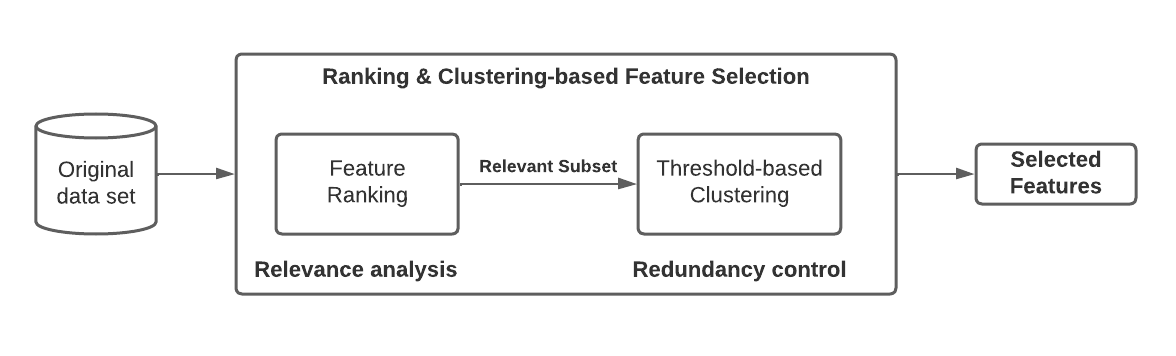
\includegraphics[width=\textwidth]{figs/etapas/Imagen1.png}
    \setstretch{1} %Interlineado 1
	\captionsetup{labelsep=period, labelfont=bf}
    \caption{Detalle de los pasos del modelo de selección}
    \label{fig:logos}
\end{figure}

\subsubsection{Análisis de relevancia}

En el proceso de clasificación, la relevancia de las características individuales se evalúa en el primer paso. Este análisis implica clasificar las características según su importancia o pesos, que son cruciales para diferenciar instancias entre diversas clases (por ejemplo, Bug o NoBug). Para este propósito, se adopta una representación específica de cada grupo, como se describe en \cite{chen_empirical_2013}.



\begin{itemize}
\item Ganancia de información (IG): La idea detrás de este algoritmo es que las características que proporcionan la mayor ganancia de información son las más útiles para la tarea de clasificación o predicción que estamos realizando.

La fórmula matemática para calcular la ganancia de información es la siguiente:

Ganancia de información = Entropía inicial - Entropía final

Donde la entropía inicial es la entropía del conjunto de datos antes de utilizar la característica para dividir el conjunto en subconjuntos más pequeños, y la entropía final es la suma de las entropías de cada subconjunto después de dividir el conjunto de datos utilizando la característica.

La entropía se calcula utilizando la siguiente fórmula:
\begin{equation}
\text{Entropía} = - \sum_{x} p(x) \log_{2}\left(p(x)\right)
	\label{eq:entropia}
\end{equation}

Donde p(x) es la probabilidad de que una observación pertenezca a la clase x.

\item Chi-Cuadrado (CS): El algoritmo Chi-Cuadrado es una técnica estadística utilizada para evaluar si existe una relación entre dos variables categóricas.

 Para calcular el valor Chi-Cuadrado, comparamos la distribución esperada con la distribución observada, es decir, con los valores reales de cada combinación de valores de A y B en nuestro conjunto de datos. Si la diferencia entre la distribución esperada y la observada es significativamente grande, podemos concluir que existe una relación entre las dos variables.

La fórmula para calcular el valor Chi-Cuadrado es la siguiente:
\begin{equation}
\text{Chi-Cuadrado} = \sum \frac{(O - E)^{2}}{E}
	\label{eq:chisqr}
\end{equation}

\item ReliefF (RF): A diferencia de otros algoritmos de selección de características, como la ganancia de información o el algoritmo Chi-Cuadrado, ReliefF tiene en cuenta la relación entre las características y las etiquetas o clases en el conjunto de datos.

El algoritmo ReliefF utiliza la distancia para evaluar cuánto aporta cada característica a la tarea de clasificación o predicción. Para ello, selecciona una observación aleatoriamente y luego busca las observaciones más cercanas y más lejanas en el espacio de características. Luego, calcula la diferencia entre la distancia a la observación más cercana y la distancia a la observación más lejana para cada característica y utiliza esta información para asignar un peso a cada característica. Las características con pesos más altos son las más importantes para la tarea de clasificación o predicción.

La fórmula matemática utilizada en el algoritmo ReliefF para asignar pesos a las características es la siguiente:

Peso de la característica i = (distancia a la observación más cercana de la misma clase - distancia a la observación más cercana de otra clase) / número de observaciones seleccionadas aleatoriamente.
\end{itemize}

\subsection{Control de redundancia}
El algoritmo de agrupamiento basado en umbrales (NTC) se utiliza para el segundo paso. En \cite{liu_empirical_2015} se encuentra un seudocódigo del algoritmo NTC.  Al principio, las funciones se agrupan en clústeres utilizando un umbral preespecificado. Para agrupar estas características, el algoritmo comienza calculando la similitud entre cada par de características y construye un gráfico de vecino más cercano sobre las características. Este proceso se repite y se van eliminando o seleccionando las características que cumplan con el umbral definido para la ejecución. Los métodos para calcular la similitud entre cualquier par de características se describirán a continuación \cite{liu_empirical_2015,chen_empirical_2013}.

\begin{itemize}
\item Incertidumbre simétrica (SU): La incertidumbre simétrica mide el coeficiente de entropía entre dos variables aleatorias y muchos investigadores la han utilizado para evaluar la similitud entre características \cite{yu2003feature,liu_empirical_2015}.
\item Semejanza de coseno (COS): La similitud de coseno mide el coseno del ángulo entre dos vectores euclidianos, construido por los valores de las dos características según el orden de instancia \cite{liu_empirical_2015}.
\end{itemize}

\subsection{Métodos de balanceo de número instancias}

\textbf{Random Under Sampling (RUS)} es una técnica de remuestreo utilizada en el aprendizaje automático para tratar el problema de desequilibrio de clases. El objetivo de RUS es reducir la cantidad de muestras de las clases sobre-representadas (o mayoritarias) de tal manera que se iguale la cantidad de muestras de las clases sub-representadas (o minoritarias) \cite{junsomboon_combining_2017,hossen_hybrid_2020}.

La manera en que se lleva a cabo el RUS es mediante la eliminación aleatoria de muestras de las clases mayoritarias. Esto se hace de forma que la proporción de muestras de las clases mayoritarias y minoritarias se acerque a una proporción deseada. Por ejemplo, si se quiere que la proporción de muestras de las clases mayoritarias y minoritarias sea 1:1, entonces se eliminarán aleatoriamente la mitad de las muestras de la clase mayoritaria.

Estas técnicas se utilizan a menudo cuando hay una desproporción significativa entre las diferentes clases en un conjunto de datos, lo que puede afectar negativamente a la precisión de los modelos de aprendizaje automático entrenados con este conjunto de datos.

En resumen, la técnica de Random Under Sampling busca balancear la proporción de muestras entre las diferentes clases reduciendo el tamaño de las clases mayoritarias.


\textbf{Random Over Sampling (ROS)} es una técnica de remuestreo utilizada en el aprendizaje automático para tratar el problema de desequilibrio de clases. El objetivo de ROS es aumentar la cantidad de muestras de las clases sub-representadas (o minoritarias) de tal manera que se iguale la cantidad de muestras de las clases sobre-representadas (o mayoritarias)  \cite{junsomboon_combining_2017,hossen_hybrid_2020}.

La manera en que se lleva a cabo el ROS es mediante la duplicación aleatoria, con reemplazo, de instancias existentes de las clases minoritarias; a diferencia de SMOTE, no crea instancias nuevas. Esto se hace de forma que la proporción de muestras de las clases mayoritarias y minoritarias se acerque a una proporción deseada. Por ejemplo, si se quiere una proporción 1:1, se duplican instancias de la clase minoritaria hasta igualar el número de instancias de la clase mayoritaria.

En resumen, la técnica de Random Over Sampling busca balancear la proporción de muestras entre las diferentes clases aumentando el tamaño de las clases minoritarias mediante la duplicación de instancias existentes.


\textbf{SMOTE (Synthetic Minority Over-sampling Technique)} es una técnica utilizada en Machine Learning para abordar el problema del desequilibrio de clases. Su objetivo es equilibrar la distribución de clases creando muestras sintéticas de la clase minoritaria. A continuación, se separa la explicación en la parte lógica matemática y el detalle del funcionamiento de SMOTE:



\textbf{Parte Lógica Matemática:}
\begin{enumerate}
\item \textbf{Detección de la Clase Minoritaria:} El primer paso es identificar la clase minoritaria en el conjunto de datos de clasificación, es decir, la clase que tiene menos ejemplos.
\item \textbf{Selección de Vecinos:} Para cada instancia de la clase minoritaria, SMOTE selecciona k vecinos cercanos. El valor de k se establece previamente.
\item \textbf{Generación de Muestras Sintéticas:} Para cada instancia de la clase minoritaria, SMOTE crea nuevas muestras sintéticas interpolando características entre la instancia original y sus vecinos seleccionados. La fórmula general es:


\begin{equation}
\fontsize{12}{9}\selectfont
\text{Nueva Muestra} = \text{Instancia Original} + (\text{Vecino} - \text{Instancia Original}) \times \text{ratio}
	\label{eq:smote}
\end{equation}

   Donde \textbf{ratio} es un valor entre 0 y 1 que determina cuánto se debe mover hacia el vecino para crear la nueva muestra.
\end{enumerate}

\textbf{Detalle del Funcionamiento:}
\begin{enumerate}
\item \textbf{Detección de la Clase Minoritaria:} SMOTE comienza identificando cuál es la clase minoritaria en el conjunto de datos. Esto se hace para asegurarse de que las nuevas muestras sintéticas se generen solo para esta clase.
\item \textbf{Selección de Vecinos:} Para cada instancia de la clase minoritaria, SMOTE elige al azar k vecinos cercanos. El valor de k se elige previamente por el usuario.
\item \textbf{Generación de Muestras Sintéticas:} Para cada instancia de la clase minoritaria, se sigue el proceso de generación de muestras sintéticas:
    \begin{enumerate}
        \item Se selecciona una instancia de la clase minoritaria.
        \item Se elige uno de sus k vecinos cercanos al azar.
        \item Se calcula un valor de 'ratio' entre 0 y 1, que determina cuánto se moverá desde la instancia original hacia el vecino. El valor de 'ratio' se elige al azar.
        \item Se utiliza la fórmula mencionada anteriormente para generar una nueva muestra sintética, que se suma a la clase minoritaria.
    \end{enumerate}
\item \textbf{Repetición:} Este proceso se repite hasta que se alcance un equilibrio deseado entre las clases o hasta que se alcance un número específico de muestras sintéticas generadas.
\end{enumerate}

SMOTE es una técnica efectiva para abordar el desequilibrio de clases, ya que aumenta el tamaño de la clase minoritaria de manera artificial, lo que puede ayudar a que los modelos de Machine Learning tengan un mejor rendimiento al tratar con datos balanceados. Sin embargo, también es importante tener en cuenta que SMOTE puede introducir ruido en los datos, ya que las muestras sintéticas se generan mediante interpolación y no representan datos reales observados. Por lo tanto, es importante evaluar el impacto de SMOTE en el rendimiento del modelo y considerar otras estrategias de manejo de datos desequilibrados según sea necesario.



\subsection{Modelos de clasificación} \label{sub:modelos}

En el estudio principal se utiliza el modelo de clasificación Random Forest (RF) en la herramienta Weka para realizar los experimentos con los diferentes conjuntos de datos. En el análisis de sensibilidad (Sección \ref{sec:sensibilidad}) se utilizan, además, XGBoost y una SVM lineal, junto con Random Forest, implementados en \textit{scikit-learn}; estos algoritmos se describen en la Sección \ref{sec:clasificadores_mt}.

RF: basado en un conjunto de árboles de decisiones. En su funcionamiento se utilizan algunas ecuaciones matemáticas, como las utilizadas en la construcción de un árbol de decisiones individual, como Gini impurity, Information Gain o Reduction in Variance \cite{shah_comparative_2020}.

La idea principal de RF es la creación de un gran número de árboles de decisiones, cada uno de ellos construido con un subconjunto de datos de entrenamiento y un subconjunto de características, y luego se combina los resultados de todos los árboles para tomar una decisión final.

El proceso de selección de características para cada árbol se realiza mediante un procedimiento conocido como "bagging" (Bootstrap Aggregating) y selección aleatoria de características, esto permite reducir la varianza y mejorar la precisión del modelo.

En resumen, el algoritmo RF se basa en la combinación de un gran número de árboles de decisiones construidos de manera aleatoria, utilizando las ecuaciones matemáticas ya mencionadas para medir la impureza o la reducción de incertidumbre en cada rama del árbol.




\newpage

